\documentclass[a4paper,oneside,onecolumn]{article}
\usepackage{graphicx}
\usepackage{amsmath}
\usepackage{amssymb}
\usepackage{subfigure}
%\usepackage{epstopdf}
\usepackage{setspace}
\onehalfspace
\usepackage{authblk}
\usepackage[margin=2.3cm]{geometry}

%\geometry{a4paper,left=2.3cm,right=2.3cm,top=2.5cm,bottom=4.5cm}
\newcommand{\nm}{\ensuremath{\,\textrm{nm}}}
\newcommand{\eV}{\ensuremath{\,\textrm{eV}}}
\newcommand{\uM}{\ensuremath{\,\mu\textrm{M}}}
\newcommand{\uW}{\ensuremath{\,\mu\textrm{W}}}
\newcommand{\meV}{\ensuremath{\,\textrm{meV}}}

\title{\textit{In situ} tuning of nanorods' plasmon through oxidative etching
with KCN}
\author[1]{Aquiles Carattino}
\author[2]{Saumyakanti Khatua}
\author[1]{Michel Orrit}
\affil[1]{Leiden Institute of Physics, Leiden, The Netherlands}
\affil[2]{Indian Institute of Technology- Gandhinagar, Ahmedabad,  India}

\begin{document}

\maketitle \abstract{The surface plasmon resonance of single-gold nanorods is of
great importance for bio-sensing, enhanced spectroscopies and photothermal
therapy. Methods for tuning this resonance after the synthesis of the
particles are of great interests for many such applications. In this work we
show that through very well known chemistry between gold and cyanide atoms it is
possible to tune the surface plasmon of individual $25\times50\nm$ rods by more
than $100\nm$ towards longer wavelengths. This is achieved by slowly etching
gold atoms from the surface of the particles, preserving their well known
optical properties.}

\section{Introduction}

Gold nanoparticles exhibit enhanced absorption and scattering cross sections
with resonances ranging from the visible to the near infra red. This property is
closely related to the surface plasmon, a collective oscillation of conduction
electrons that depends on the shape of the particles. For gold nanorods (AuNR)
the surface plasmon resonance (SPR) energy depends on the aspect ratio (AR) of
the particle and can be found between $550\nm$ for spheres (AR of $1$) to beyond
$800\nm$ for elongated particles.

The surface plasmon presents great opportunities in (bio-)
sensing\cite{Zijlstra2012}, enhanced spectroscopies\cite{Sivapalan2013},
photothermal therapy\cite{Zhao2014}, and for concentrating light below the
diffraction limit\cite{Zijlstra2011}. Success in many of these applications
requires precise and in situ control over the nanoparticles' plasmon resonance
energy. For example, maximum fluorescence\cite{Khatua2014} or Raman
enhancement\cite{McFarland2005} is achieved when the nanoparticle's plasmon
resonance is tuned to the excitation laser wavelength or efficient photothermal
therapy requires the nanoparticles' SPR to be tuned to NIR to minimize the
damage to healthy cells\cite{Alkilany2012}.

Typically, the SPR is tuned by carefully manipulating the shapes of
nanoparticles during their synthesis. Particularly useful are the rod-shaped
particles, whose resonance can be tuned from $600\nm$ to over $1000\nm$ by
changing their aspect ratios through carefully adjusting the concentrations of
gold-seed and silver nitrate during the seed-mediated growth synthesis
method\cite{Vigderman2012}. Many other nanoparticles shapes, such as nanoprisms,
nanorice, nanocubes, nanoshells, etc. have been synthesized with their plasmon
resonances covering the entire spectral range from visible to
near-IR\cite{Lal2007}. Wet-chemical synthesis methods, however, generally yield
a broad distribution in nanoparticle sizes and/or shapes, which hinders precise
and reproducible tuning of nanoparticle SPR. Furthermore these methods do not
provide any in-situ adjustment of the SPR; any change of which requires a new
synthesis.

Recently, new methods have been developed to tune nanoparticle SPRs after their
synthesis. These approaches can be divided into two broad categories: ($1$) The
first group of methods tune the refractive index of the medium using an electric
or magnetic field\cite{Kossyrev2005}. The advantage of these methods is that the
SPR shift is reproducible and reversible. However the tuning range is rather
limited and continuous tuning within this range is difficult to achieve.
($2$) The other set of approaches rely on controllably inducing shape
modifications of the nanoparticles to tune the plasmon resonance through
chemical or physical means. For example, thermal reshaping was induced by
illuminating the nanoparticles with an intense, pulsed
\cite{Link2000}\cite{Horiguchi2008} or continuous laser\cite{Yorulmaz2012}.
Increasing the particles' temperature therefore leads to changes in shape,
favoring those conformations with a lower surface energy (i.e.
spheres over rods, etc.). Chemical reshaping is also possible and was the focus
of several studies\cite{Carbo-Argibay2007}
\cite{Rodriguez-Fernandez2005} \cite{Jana2002}. In those cases, the capping
agent will induce different reactivities on the sides than on the tips of the
particles; because of a higher curvature\cite{Yuan2015} the tips are
normally more susceptible to chemical reactions, leading to an anisotropic reshaping
shortening the long axis or softening any high-curvature region. In both cases
(laser or chemical induced reshaping) the outcome is a blue-shift of the surface
resonance peak.

Here we present a new approach for precise and in-situ tuning of plasmon
resonances of single gold nanorods isolated and immobilized over a glass
surface. A nanorod's plasmon resonance is tuned over $130\nm$ (starting from
$650\nm$ up to $780\nm$). Our method exploits well known chemistry between gold
and potassium cyanide (KCN), to controllably etch gold atoms from the
nanoparticle and thereby change its aspect ratio. We note that unlike many of
the previous studies, here we observe a SPR red shift on gold nanorods.
Our simulations based on the discrete dipole approximation method attributes
this red shift to isotropic etching of gold nanorods from all sides resulting in
an overall increase of aspect ratio.  This is also verified from scanning
electron microscopy (SEM) images and results contrary to previous studies, where
the etching was preferred at the tips, yielding in an overall increase of
aspect ratios.

\section{Experimental method}

\begin{figure}[p]
 \centering 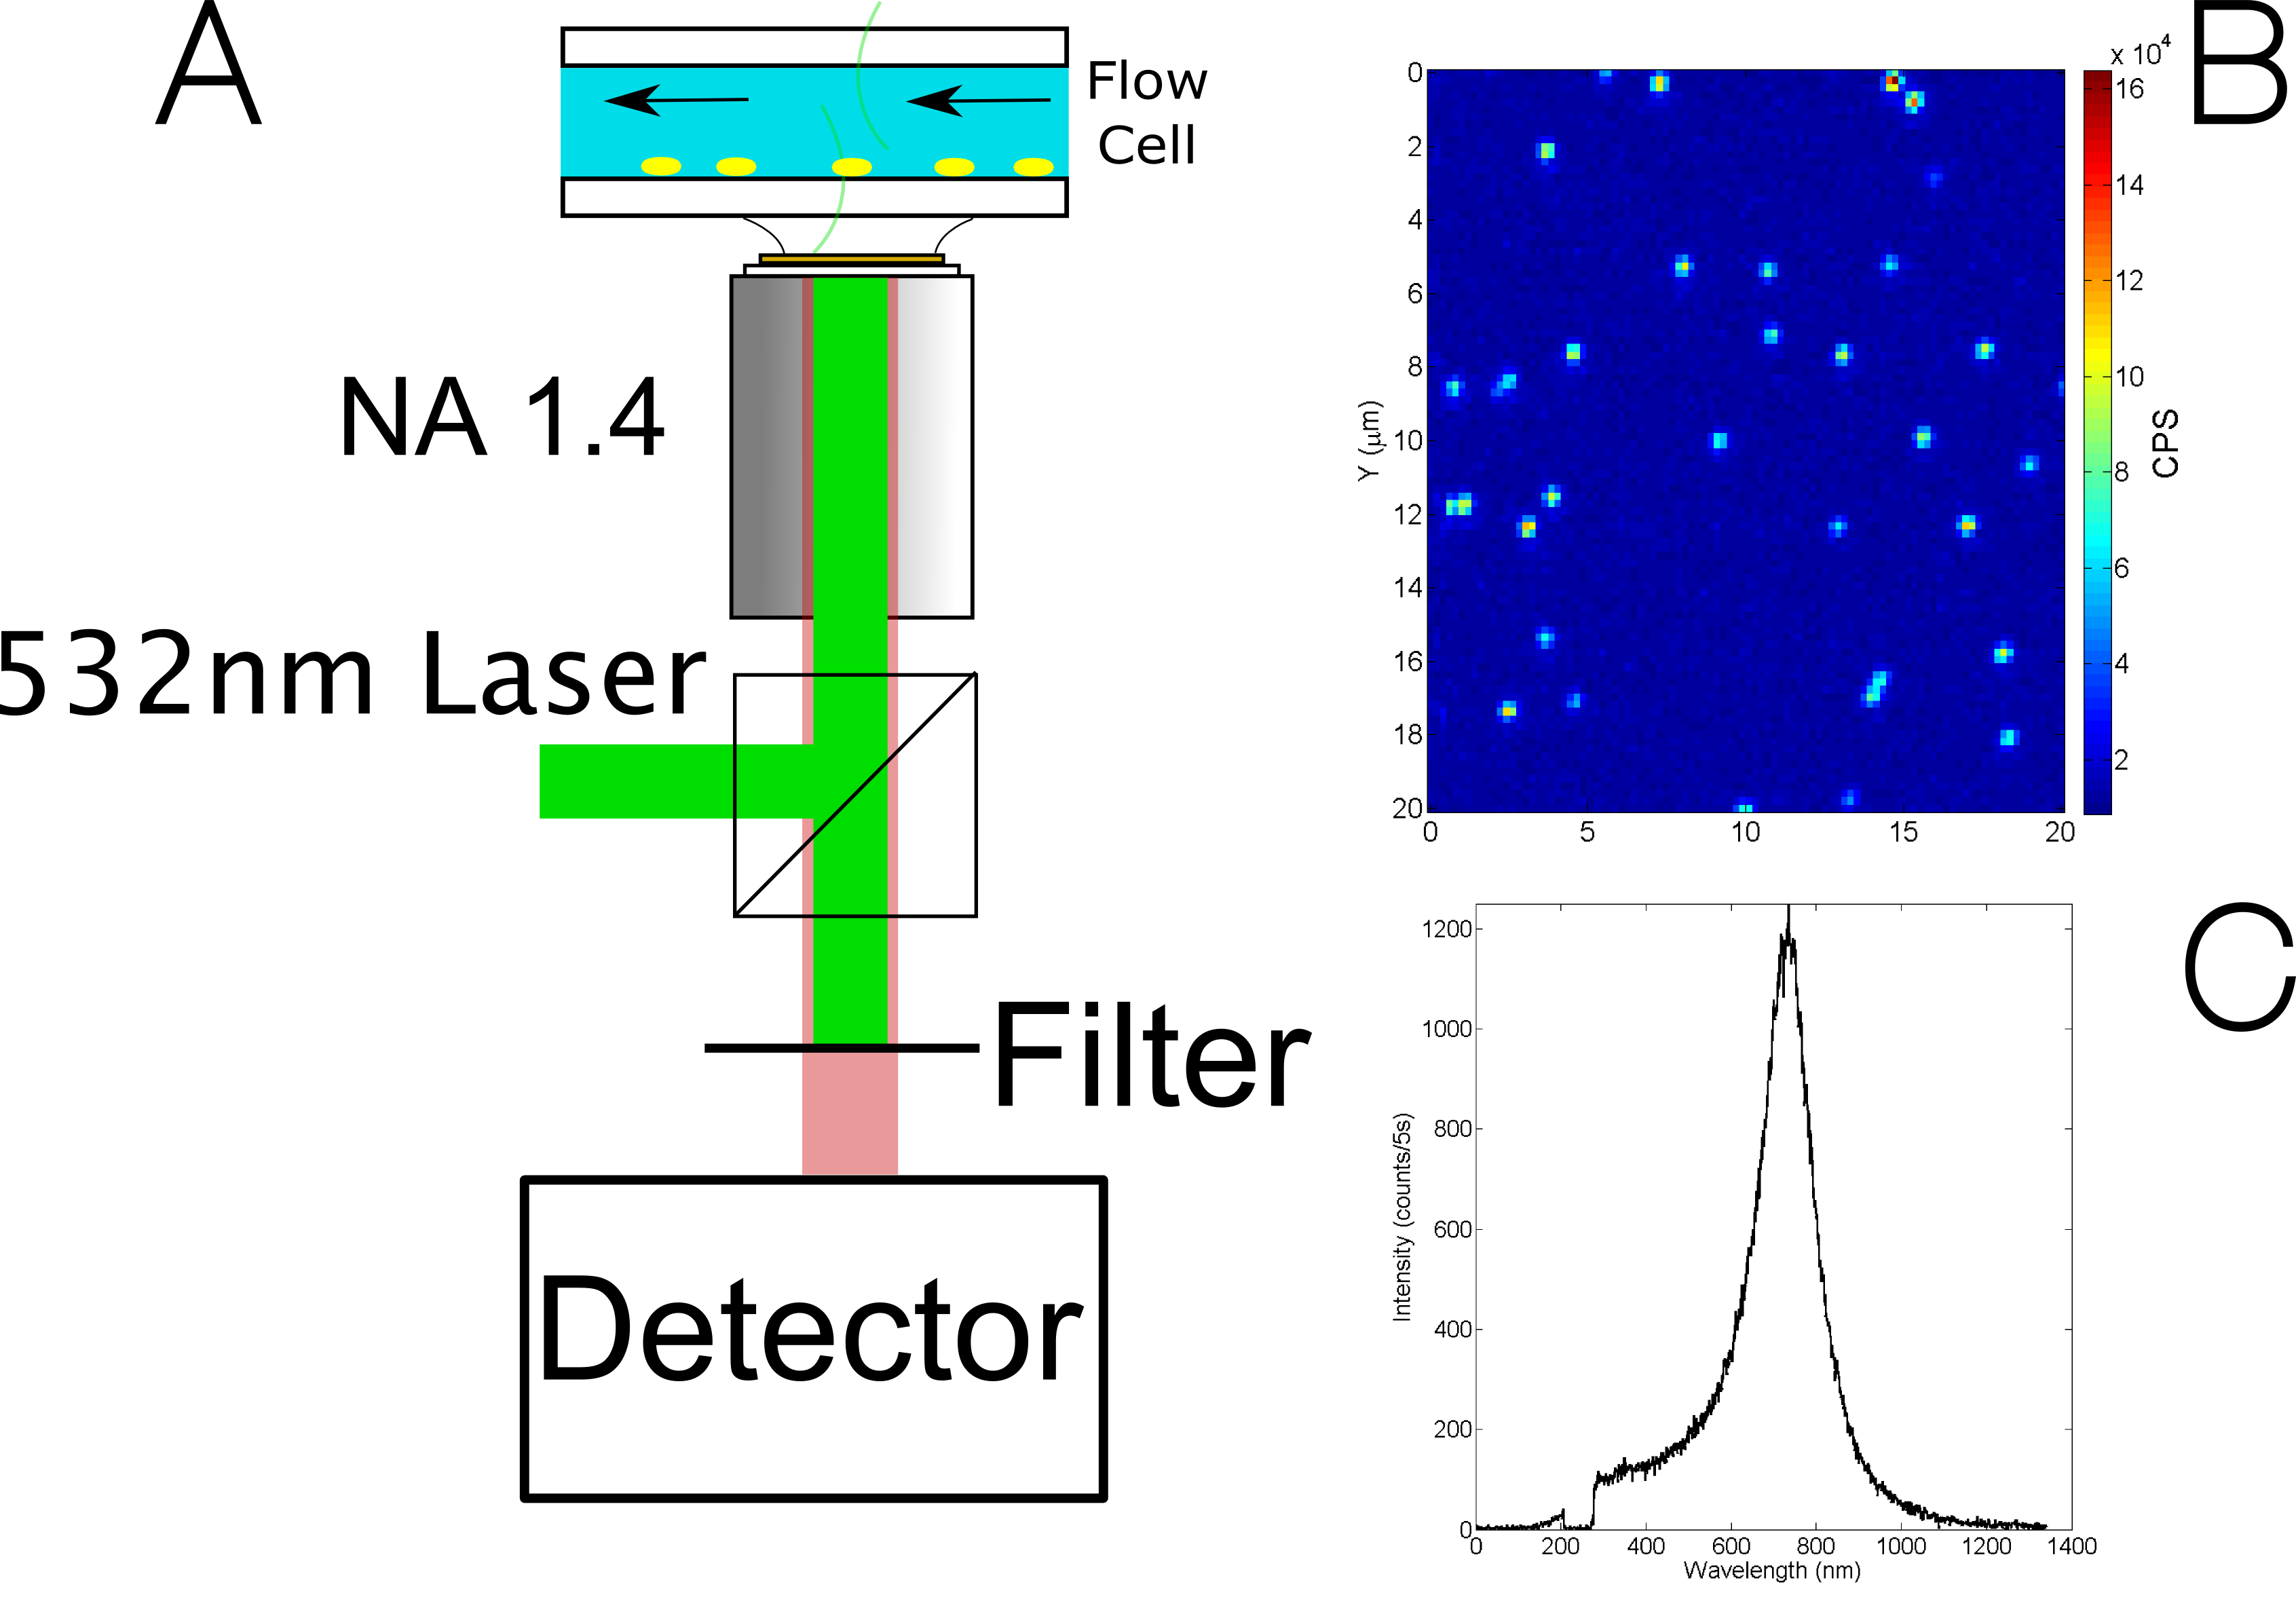
\includegraphics[width=0.45\linewidth]{Figures/01_Setup/setup_1.png}
 \caption{Experimental setup and examples of observations. a) Simplified
 schematic of the confocal microscope employed during the measurements. b) A
 typical 1-photon luminescence raster scan of the sample immersed in
 water, before etching and c) luminescence spectrum of a single rod.}
 \label{fig:setup}
\end{figure}

Gold nanorods were synthesized by following standard seeded growth
methods\cite{Nikoobakht2003}. The average size of the nanorods was $50\nm\times
25\nm$ and their SPR is located at $650\nm$ in water (refer to the
supplementary material for the SEM image and bulk extinction of nanorods as
synthesized).

Single-particle measurements were done on a home-built confocal microscope
(Figure \ref{fig:setup}a). A $532\nm$ laser was used for exciting the particles.
The excitation power was $300\uW$ at the back focal plane of the objective
(Olympus $60\times$, $\textrm{NA}\,0.9$ air). The luminescence signal was then
filtered with two $532\nm$ notch filters and was detected by either an avalanche
photodiode or a liquid nitrogen-cooled CCD-spectrometer (Acton $500\textrm{i}$).
The images were acquired by scanning the sample across a tightly focused laser
beam using a XYZ piezo scanning stage (PI Nano Cube).

The samples were prepared by spin casting a suspension of AuNR on clean
coverslips and thoroughly rinsing them  with Milli-Q water and placed in an
ozone cleaner for eliminating the excess of CTAB. Afterwards the samples are
placed in a flowcell; the initial spectra are taken with the rods immersed in
Milli-Q water (see for example Figure \ref{fig:setup}c). This initial
characterization allows us to discard clusters of rods\cite{Funston2009}.
Next, a solution of KCN was flowed into the cell with concentrations ranging
from $3\uM$ to $80\uM$. In each case the spectra of approximately $10$
different particles are acquired consecutively after focusing on each one. The
time resolution varies according to the exposure time and number of particles;
in this work a spectra of each particle is taken at least every minute.

\section{Results}

Figure \ref{fig:setup}b shows a typical one-photon-excited luminescence image
of gold nanorods isolated on a glass surface and covered with water.
Approximately $90\%$ of the diffraction-limited bright spots originate from
single gold nanorods. This was confirmed by acquiring their luminescence
spectra; a typical result is shown in Figure \ref{fig:setup}c which shows
a narrow Lorentzian lineshape\cite{Funston2009}.

\begin{figure}[p]
 \centering
 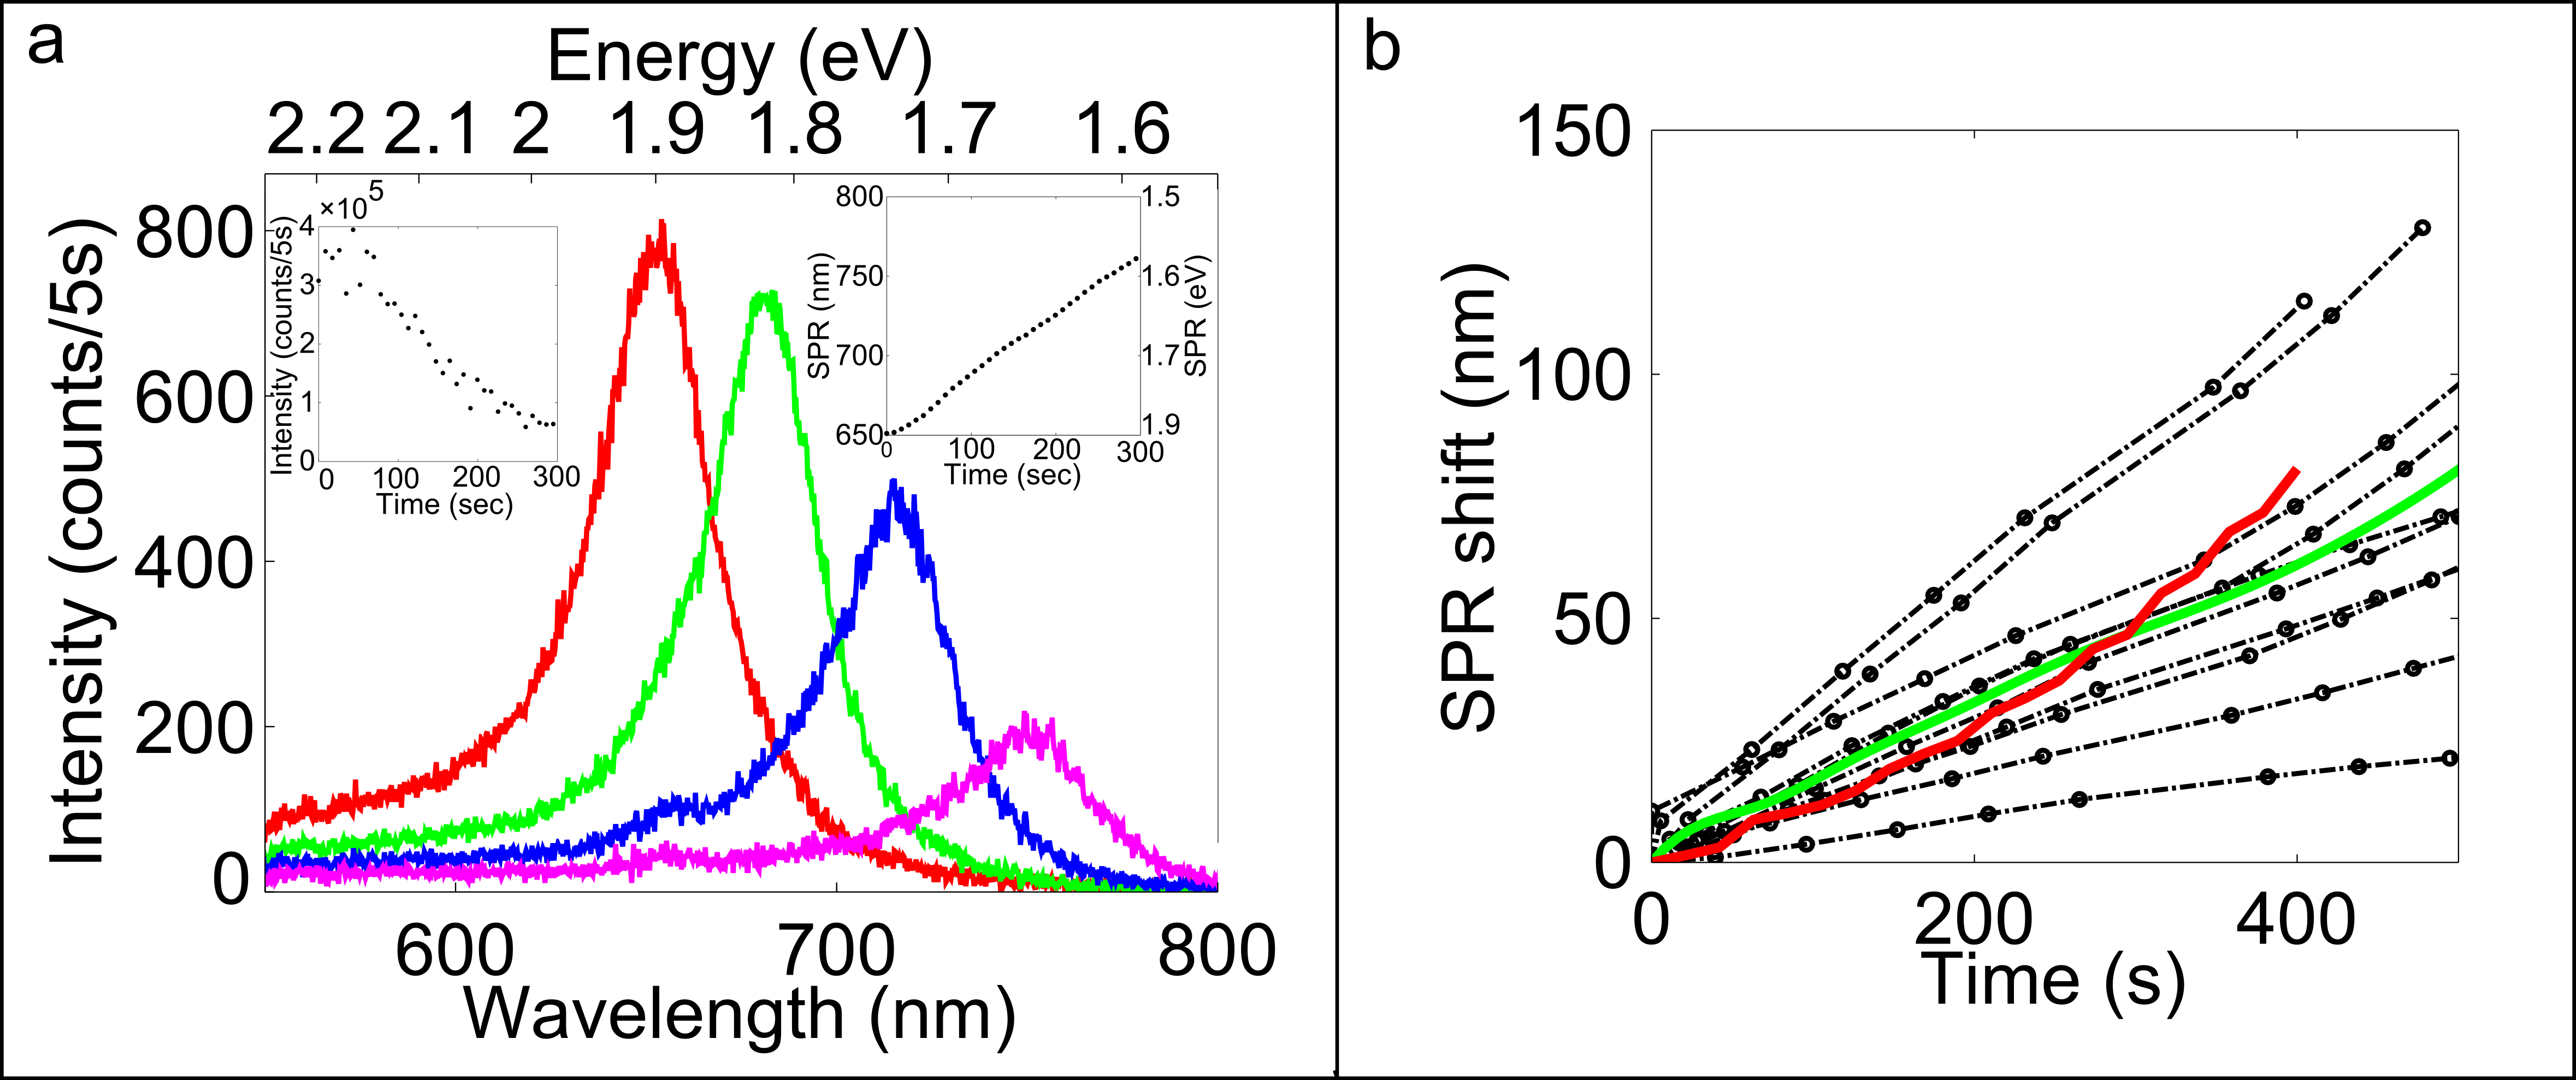
\includegraphics[width=0.95\linewidth]{Figures/02_Experimental/Experimental.png}
 \caption{One photon luminescence spectra of gold nanorods immersed in $20\uM$
 KCN. a) Plasmon shift of a single rod. The curves are displayed at $70s$
 intervals. The insets display the intensity of the peak and the resonance
 wavelength as a functions of time respectively. b) The peak shift time-trace
 for 9 different particles. The red curve is the average while the green is the
 best fit from discrete dipole simulations with etching rate fixed at
 $1\nm/\textrm{min}$}
 \label{fig:plasmon_single_rod}
\end{figure}

Figure \ref{fig:plasmon_single_rod}a shows the one-photon luminescence spectra
of a gold nanorod immersed in $20\uM$ KCN at intervals of $70\,\text{s}$. We
clearly observe a gradual red-shift of the nanorod's plasmon resonance by more
than  $100\nm$ over a time interval of $300\,\text{s}$. This red-shift is also
associated with a decrease of photoluminescence intensity by factor of $4$. A
more detailed analysis shows that the nanorod's plasmon resonance wavelength
(calculated from fitting with a lorentzian function) varies almost linearly
with respect to time (inset of Figure \ref{fig:plasmon_single_rod}a). We note
the presence of an additional shoulder peak at $650\nm$ ($1.9\,\eV$) which is
more prominent for the less intense curves and is due to Raman scattering of
water\cite{Snow1985} that could not be completely removed when subtracting the
background (see SI for the spectra of the background).

We find the same trend for all the nanorods that were studied. Our results are
summarized in Figure \ref{fig:plasmon_single_rod}b, which shows the shift of
plasmon resonance wavelengths as a function of time for nine different rods
(dashed lines). Each nanorod shows a red-shift of the plasmon resonance
wavelength which varies almost linearly with time irrespective of their
initial resonance energy. The rate of SPR shift however, varies significantly
from particle to particle, the hoghest rate was $15\nm/\textrm{minute}$
while the lowest one was $2\nm/\textrm{minute}$. The green curve in Figure
\ref{fig:plasmon_single_rod}b is the average of all the shifts; since the
spectra of each particle were acquired sequentially, we interpolated the
values of the shift at intermediate times with a cubic spline.

The reaction between gold and potassium cyanide is well known and is being used
for gold mining, electroplating, organic synthesis, etc. Gold reacts with
aqueous CN$^-$ ions in presence of oxygen to form $\textrm{Au(CN)}_2^-$, which
is soluble in water. The reaction can be written as follows
\begin{equation*}
4\textrm{Au} + 8\textrm{CN}^-+\textrm{O}_2 + 2\textrm{H}_2\textrm{O}
\leftrightarrows 4\textrm{Au(CN)}_2^-+4\textrm{OH}^- \end{equation*} 
In our experiment the formation of $\textrm{Au(CN)}_2^-$ results in gold etching from the nanorods, as has been reported previously\cite{Jana2002}.

The etching of gold atoms from a nanorod has two effects: Firstly, the
nanorods' volume will decrease gradually with longer reaction time. This is
consistent with our observation that the one-photon-luminescence intensity
decreases with time. Secondly, the aspect ratio of a nanorod can either
decrease or increase depending on the preferred direction of etching.
Nanorod aspect ratio will decrease with time when the reaction happens
preferably at the tips. This is indeed the case for nanorods protected with
CTAB and dispersed in solution\cite{Jana2002}. CTAB binds weakly to the tips
compared to the sides and therefore leaves the tips more susceptible for
chemical reactions\cite{Caswell2003}. The consequent decrease of aspect ratio
yields a blue shift of the plasmon resonance\cite{Link1999}. In a second case,
etching happens isotropically from both sides and tips resulting in an overall
increase of the nanorod's aspect ratio. This is the more likely scenario in
our experiment as the nanorods' surface does not have any protective CTAB bilayer.

Numerical simulations based on the discrete dipole approximation were
performed to further confirm that the red shift of the plasmon resonance is
indeed due to isotropic etching of the nanorods. The initial dimensions of the
particles were fixed at $25\nm\times50\nm$ which coincided with the median
dimensions of the distribution of sizes of the nanoparticles (see SI). These
simulations are carried out in steps of $0.5\nm$ for a total of $10\nm$ (i.e.
the minimum particle size is $15\nm\times 40 \nm$). Figure
\ref{fig:simulations}a shows the scattering spectra of the particle at
different etching intervals. We clearly observe a red-shift of the plasmon
resonance wavelength, as was observed in our experiment. The insets of the
figure show the decrease of the integrated scattering spectrum as a function of
the etching and the detailed time-evolution of the SPR obtained from the fitting
of the peaks with a lorentzian function. Both are compatible with the
experimental observations. Furthermore it is possible to fix the etching rate to
best approximate the average plasmon shift. These results are displayed as the
red curve in Figure \ref{fig:plasmon_single_rod}b. The best approximation to
the average is found when the etching rate is set to $1\nm/\textrm{min}$. 

\begin{figure}[p]
 \centering
 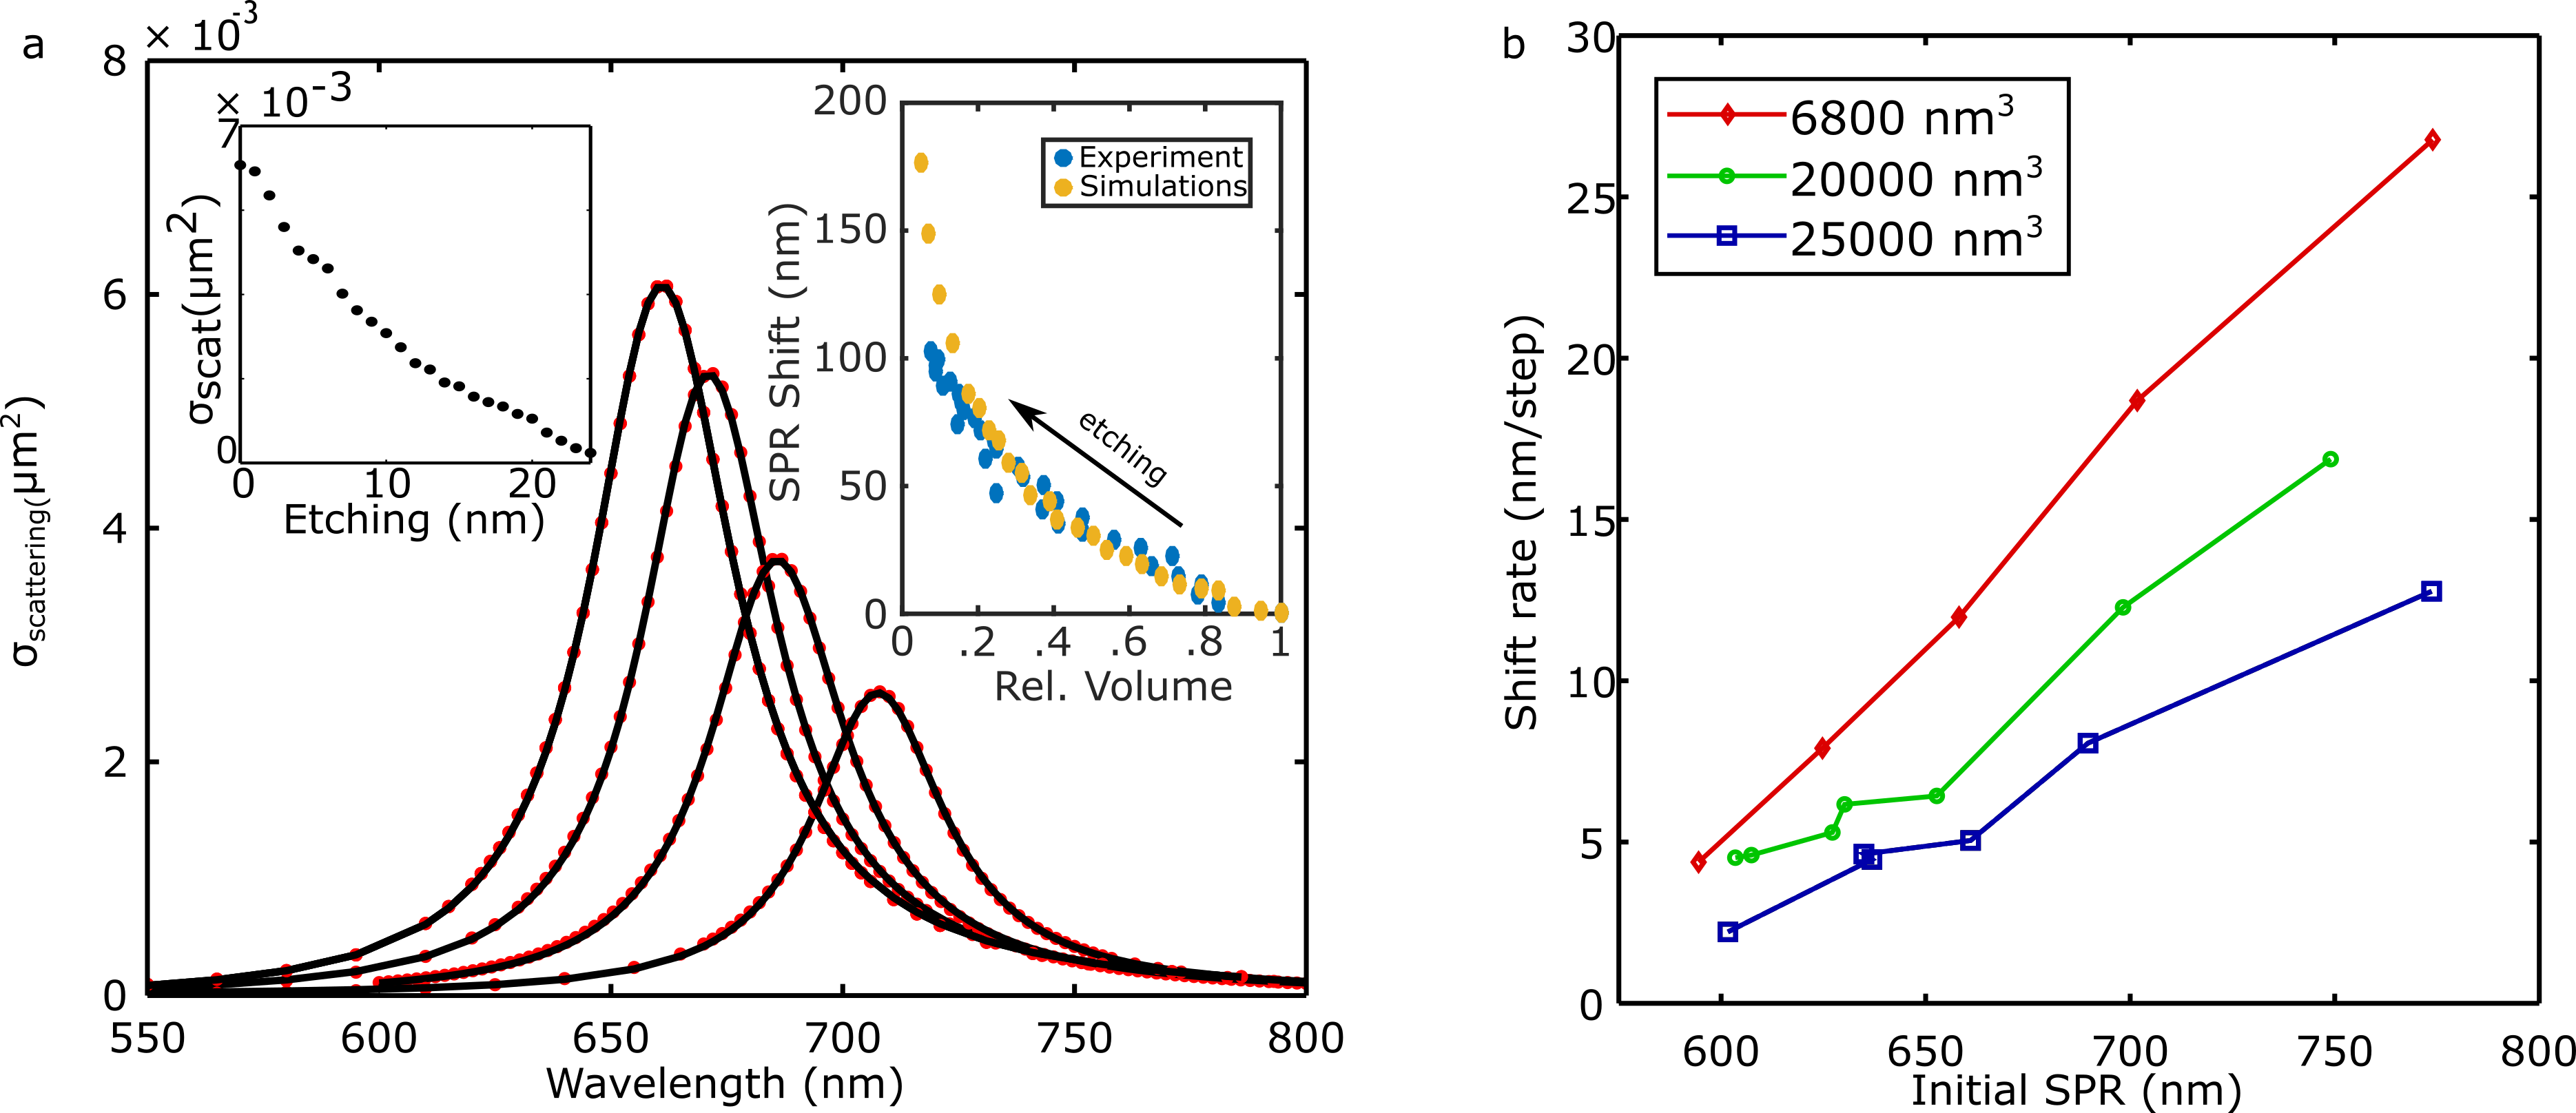
\includegraphics[width=0.95\linewidth]{Figures/02_Simulations/simulations.png}
 \caption{Simulated plasmon spectra at different etching steps. a) Examples of
 the curves obtained at different simulations steps. The black curves are
 fittings with lorentzians. The insets show the intensity and the SPR as
 functions of the etching. b) Shift rate as a function of the initial
 plasmon resonance. The size of the markers is proportional to the initial
 volume of the rods.}
 \label{fig:simulations}
\end{figure}

Furthermore the simulations allow us to study the different shift rates that
were present in the experimental results. Figure \ref{fig:simulations}b shows the
different shift rates as functions of the initial plasmon resonance of different
particles. In this case the initial sizes ranged from $45\nm\times25\nm$ to
$90\nm\times37\nm$. The shift rate is defined through a linear fit of the
plasmon shift as a function of the amount of etching. The size of the markers of
each particle denote their volume (the smallest being $1.8\times10^4\nm^3$ and
the largest $8.4\times10^4\nm^3$. In this way it is possible to observe that
particles with the same (or similar) volume, have faster shift rates if their
initial aspect ratio is larger (i.e. the SPR is red-shifted.) On the other hand,
particles with a similar initial resonance, show a faster shift if they are
smaller. 

\begin{figure}[p]
 \centering
 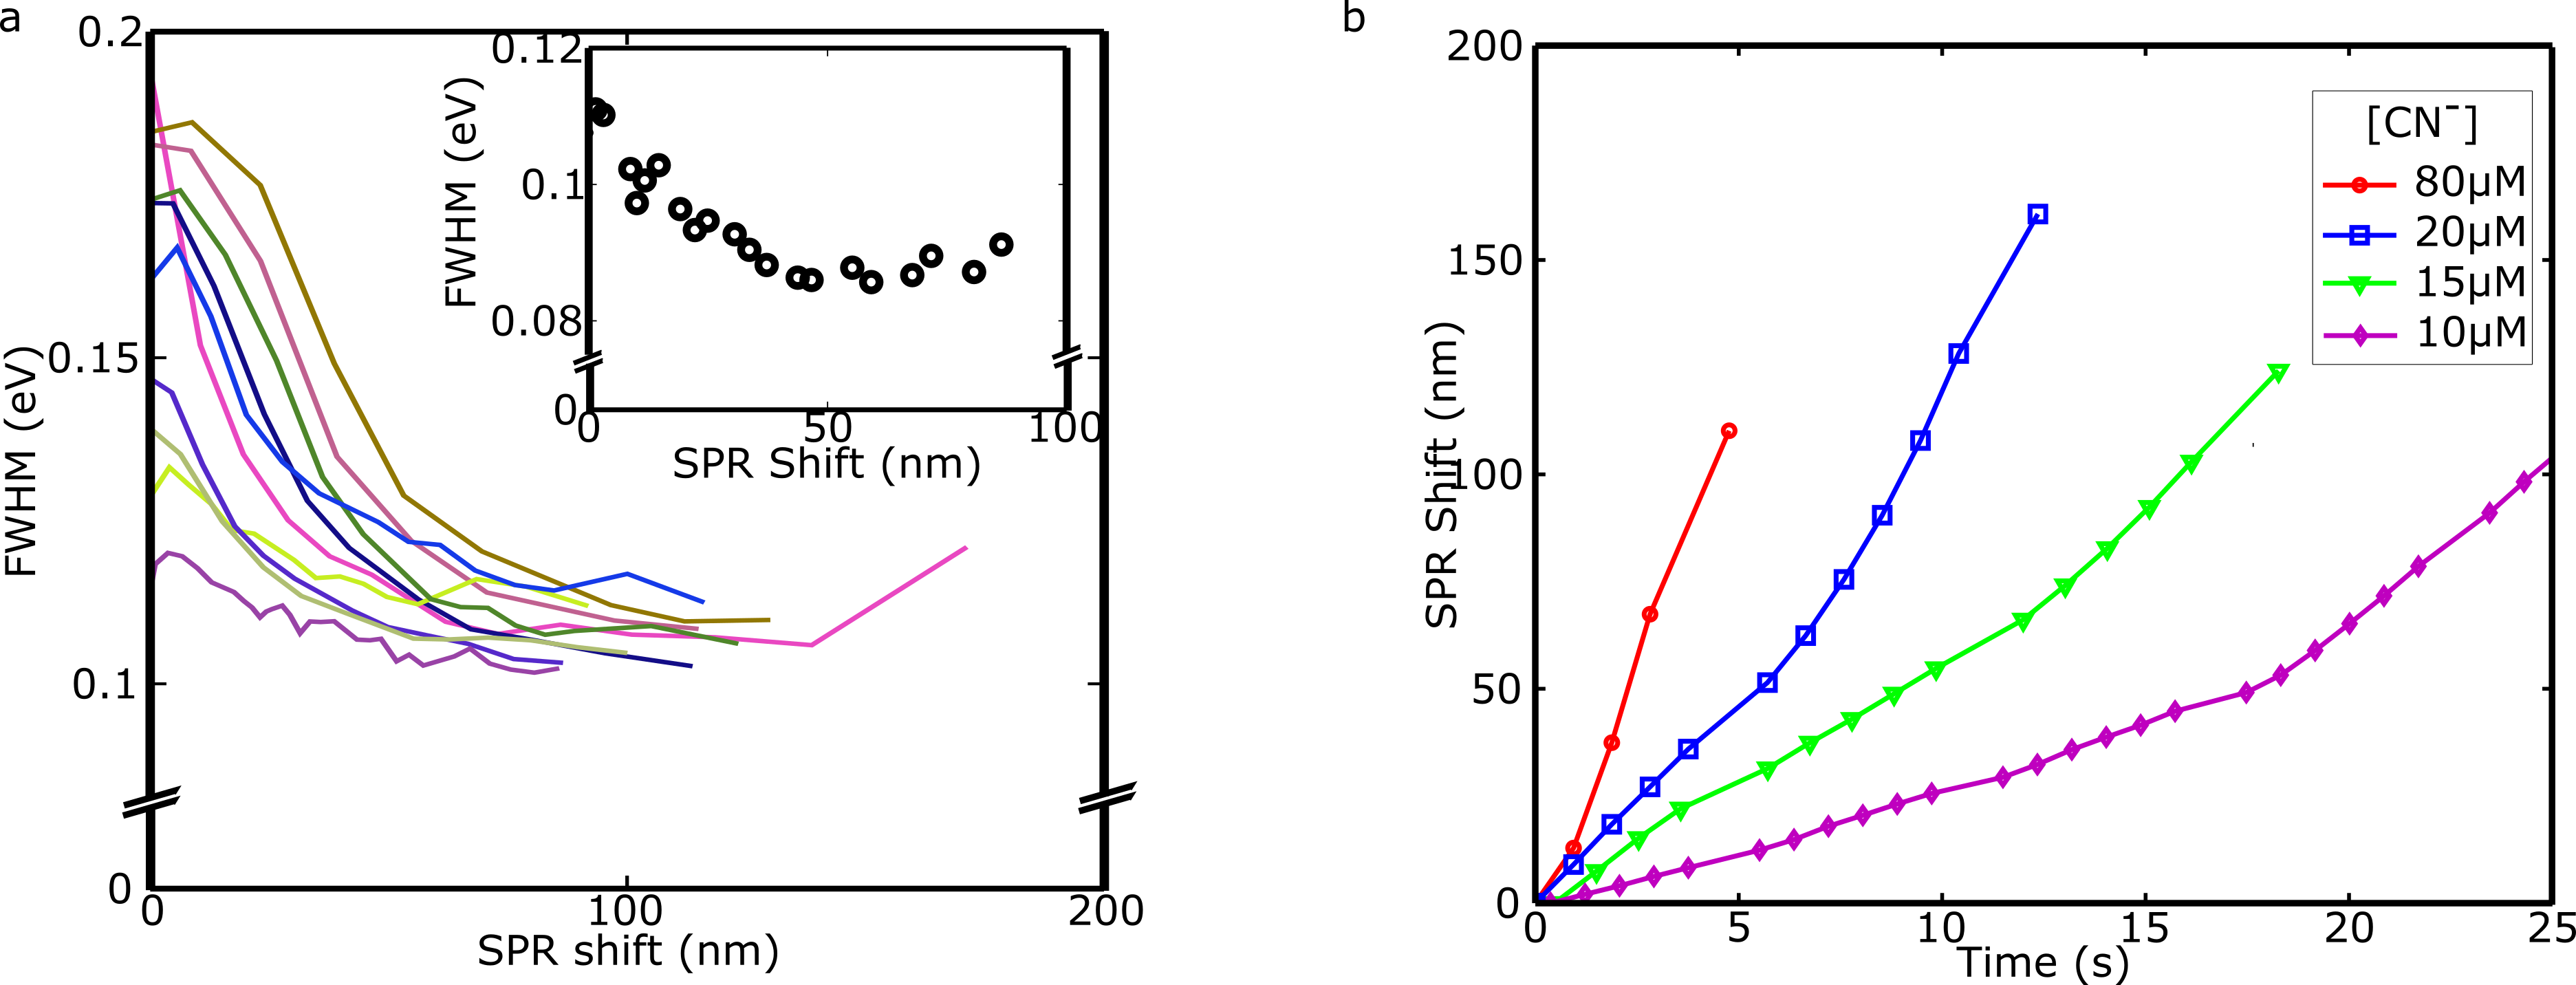
\includegraphics[width=0.95\linewidth]{Figures/03_Shifts/shifts.png}
 \caption{a) Plasmon FWHM of different particles immersed in $20\uM$
 KCN as a function of their plasmon shift. The inset shows the results from the
 simulations carried out with the ADDA package. b) SPR Shift as a function of
 time for particles with the same initial SPR at different KCN concentrations.}
 \label{fig:FWHM}
\end{figure}

Figure \ref{fig:FWHM}a shows how the FWHM of the plasmon peak decreases while
the shift increases for several nanorods immersed in $20\uM$ KCN. Note that the
plot shows the width of the resonance in units of energy and not in units of
wavelength. Because of the nonlinear relation between them, the peak width
expressed in wavelength depends on the peak position rendering impossible the
comparison of widths during the shift. At the beginning of the reaction there is
a rapid diminishing of the width. Then a minimum is reached for shifts between
$75\nm$ and $100\nm$. After this point the volume of the particles is highly
reduced, and therefore their luminescence intensity and it is not possible to
reliably extract information from the spectra. The inset of the Figure shows
the FWHM obtained from the simulations for a $25\nm\times50\nm$ nanorod. The
width decreases with the shift slightly slower than in the experiment but the
trend is similar to the observed one.

The faster decrease of the resonance FWHM observed in the experiments as
compared to the simulations may be due to the elimination of defects from the
surface of the particles. However, the overall observed and simulated decrease
of width can be explained considering that both the radiative and non-radiative
damping decrease during the etching process. The radiation damping scales as the
volume of the particle\cite{Wokaun1982} and therefore will decrease while the
cyanide etches gold atoms from the particle.
On the other hand, we observe that the energy distance between the longitudinal
plasmon peak and interband transitions in gold increases during the etching
process. Therefore the non-radiative damping mechanisms in the particle become
less efficient\cite{Sonnichsen2002}. These effects combined may therefore have a
role in the diminishing plasmon width that is observed.

Figure \ref{fig:FWHM}b shows the plasmon peak shift as a function of time for
various KCN concentrations for particles with a plasmon peak position of
roughly $630\nm$. As shown for the simulations (Figure
\ref{fig:simulations}b), the initial SPR will have a role on the etching rate,
therefore it is important to choose particles that are similar to each other.
The time-traces of the peak position clearly show that the shift rate is
proportional to the concentration of KCN. It is important to note that the
behavior of the FWHM in all the cases is similar and it resembles the results
shown in Figure \ref{fig:FWHM}a. This means that the shift rate does not have an
effect on the quality of the plasmon resonance.

By fitting the simulations to the experimental results it is possible to
estimate the volume of gold etched away from a particle by unit of time.
Assuming an atomic radius of gold of $144\,\textrm{pm}$\cite{Pauling1947} we
obtain that for a KCN concentration of $10\uM$ the reaction rate can be as low
as $700$ atoms per second. From the simulations and these estimates it is
possible to approximate the plasmon shift for every etched atom. In the same
conditions as before, it would be $0.2\cdot 10^{-3}\, \textrm{nm}/
\textrm{atom}$. This is several orders of magnitude smaller that the sensitivity
of our experiments. 

Samples of the same nanorods are prepared for SEM imaging by drop casting the
same solution of rods. The images were acquired before the etching, after
$2\,\textrm{min}$ immersion in KCN and after $4\,\textrm{min}$. In each case we
observed that when particles are isolated from each other, the rod-shape is
preserved; for aggregates of particles this no longer holds, and rods start to
lose their shape (see Supporting Information for SEM images.) Calculating the
distribution of sizes of the particles shows a slight increase in the aspect
ratio but this is obscured by the broad distribution of values, even before
starting the etching.

The same experiments performed in bulk (see SI) show a different behaviour of
the plasmon resonance. As reported by other groups \cite{Jana2002}
\cite{Yuan2015}, the rods reshape into spheres and this can be explained by the
presence of CTAB: the tips will be more exposed and therefore react more
quickly, yielding a net decrease in aspect ratio. In our single-particle
experiments the CTAB was removed but now there is the glass surface supporting the rods that has
to be taken into account. In principle there is a side of the rods in contact
with the surface that will be less exposed to KCN; the etching in this case
wouldn't be isotropic and would flatten the rods. Neither the optical nor the
SEM images allow us to assess this question because there is no information on the
third axis (perpendicular to the surface). Experiments performed in an optical
tweezer away from the surface as done in Ref \cite{Ni2012} but without the
capping agent would involve in addition the use of microfluidics and therefore
are much harder to perform.

\section{Conclusions}

In this work we have shown a simple method that allows us to tune the plasmon
peak position of single gold nanorods with nanometer accuracy and over the
range of $100\nm$ ($300\meV$). More importantly, we show that during the
etching process the rod-like shape is preserved; this was confirmed both by
monitoring the FWHM of the resonance peak and by acquiring SEM images after
different reaction times. The experiments allowed us to record the plasmon
peak with a relatively high temporal and spectral accuracy, allowing us to
stop the reaction when the resonance is at the desired value.

The ADDA simulations with the isotropic etching model allowed us to estimate
the amount of gold being etched from the nanoparticles. They were consistent
in both predicting the red-shift of the plasmon and the diminishing intensity
of the luminescence signal. SEM images of the rods confirmed the values
obtained from the simulations. Combining these results provide a way of
predicting the behaviour of the plasmon peak for different rods.

We observed a broad distribution of the rate at which the plasmon peak shifts
for different particles under the same experimental conditions. This can be
attributed to the initial aspect ratios and volumes of each particle. Sphere-
like particles will show a small shift due to the fact that the aspect ratio
is constant while under isotropic etching. The more elongated particles, on
the other hand, will have a much steeper increase in aspect ratio while being
etched. Also intrinsic differences between the particles, for instance the
faceting of the surface, or the prescence of left over CTAB that was not
completely washed away can also cause different results and are much harder to
quantify.

The role of the capping agent has largely been studied and has always been
held responsible for the observations both in chemical etching\cite{Yuan2015}
and for photothermal reshaping\cite{Horiguchi2008}. Avoiding the presence of
the passivating layers is impossible in suspension, since gold nanoparticles
would aggregate. Our results provide evidence that supports previous
observations regarding the effect of the curvature and the accessibility of
KCN to the surface of the particle. 

\bibliography{bibliography}{}
\bibliographystyle{ieeetr}

\end{document}
